\documentclass{article}

% Language setting
% Replace `english' with e.g. `spanish' to change the document language
\usepackage[english]{babel}
\usepackage{float}

% Set page size and margins
% Replace `letterpaper' with `a4paper' for UK/EU standard size
\usepackage[letterpaper,top=2cm,bottom=2cm,left=3cm,right=3cm,marginparwidth=1.75cm]{geometry}

% Useful packages
\usepackage{amsmath}
\usepackage{graphicx}
\usepackage[colorlinks=true, allcolors=blue]{hyperref}

\title{PS6 DScourse 2024}
\author{Emilien Akotenou}

\begin{document}
\maketitle
\section{Data}
The data set contains information on the performance and characteristics of all Premier League players. For instance, the data has information on the player's team, the number of goals per match.

\section{Descriptive statistics}
\subsection{English Premiere League's players performance}
The figure 1 presents the number of goals scored by player as function of being in their preferred team. Clearly,it appears that players perform highly when being in their dream team. They scored on average 13 goals per season.

\begin{figure}[H]
\centering
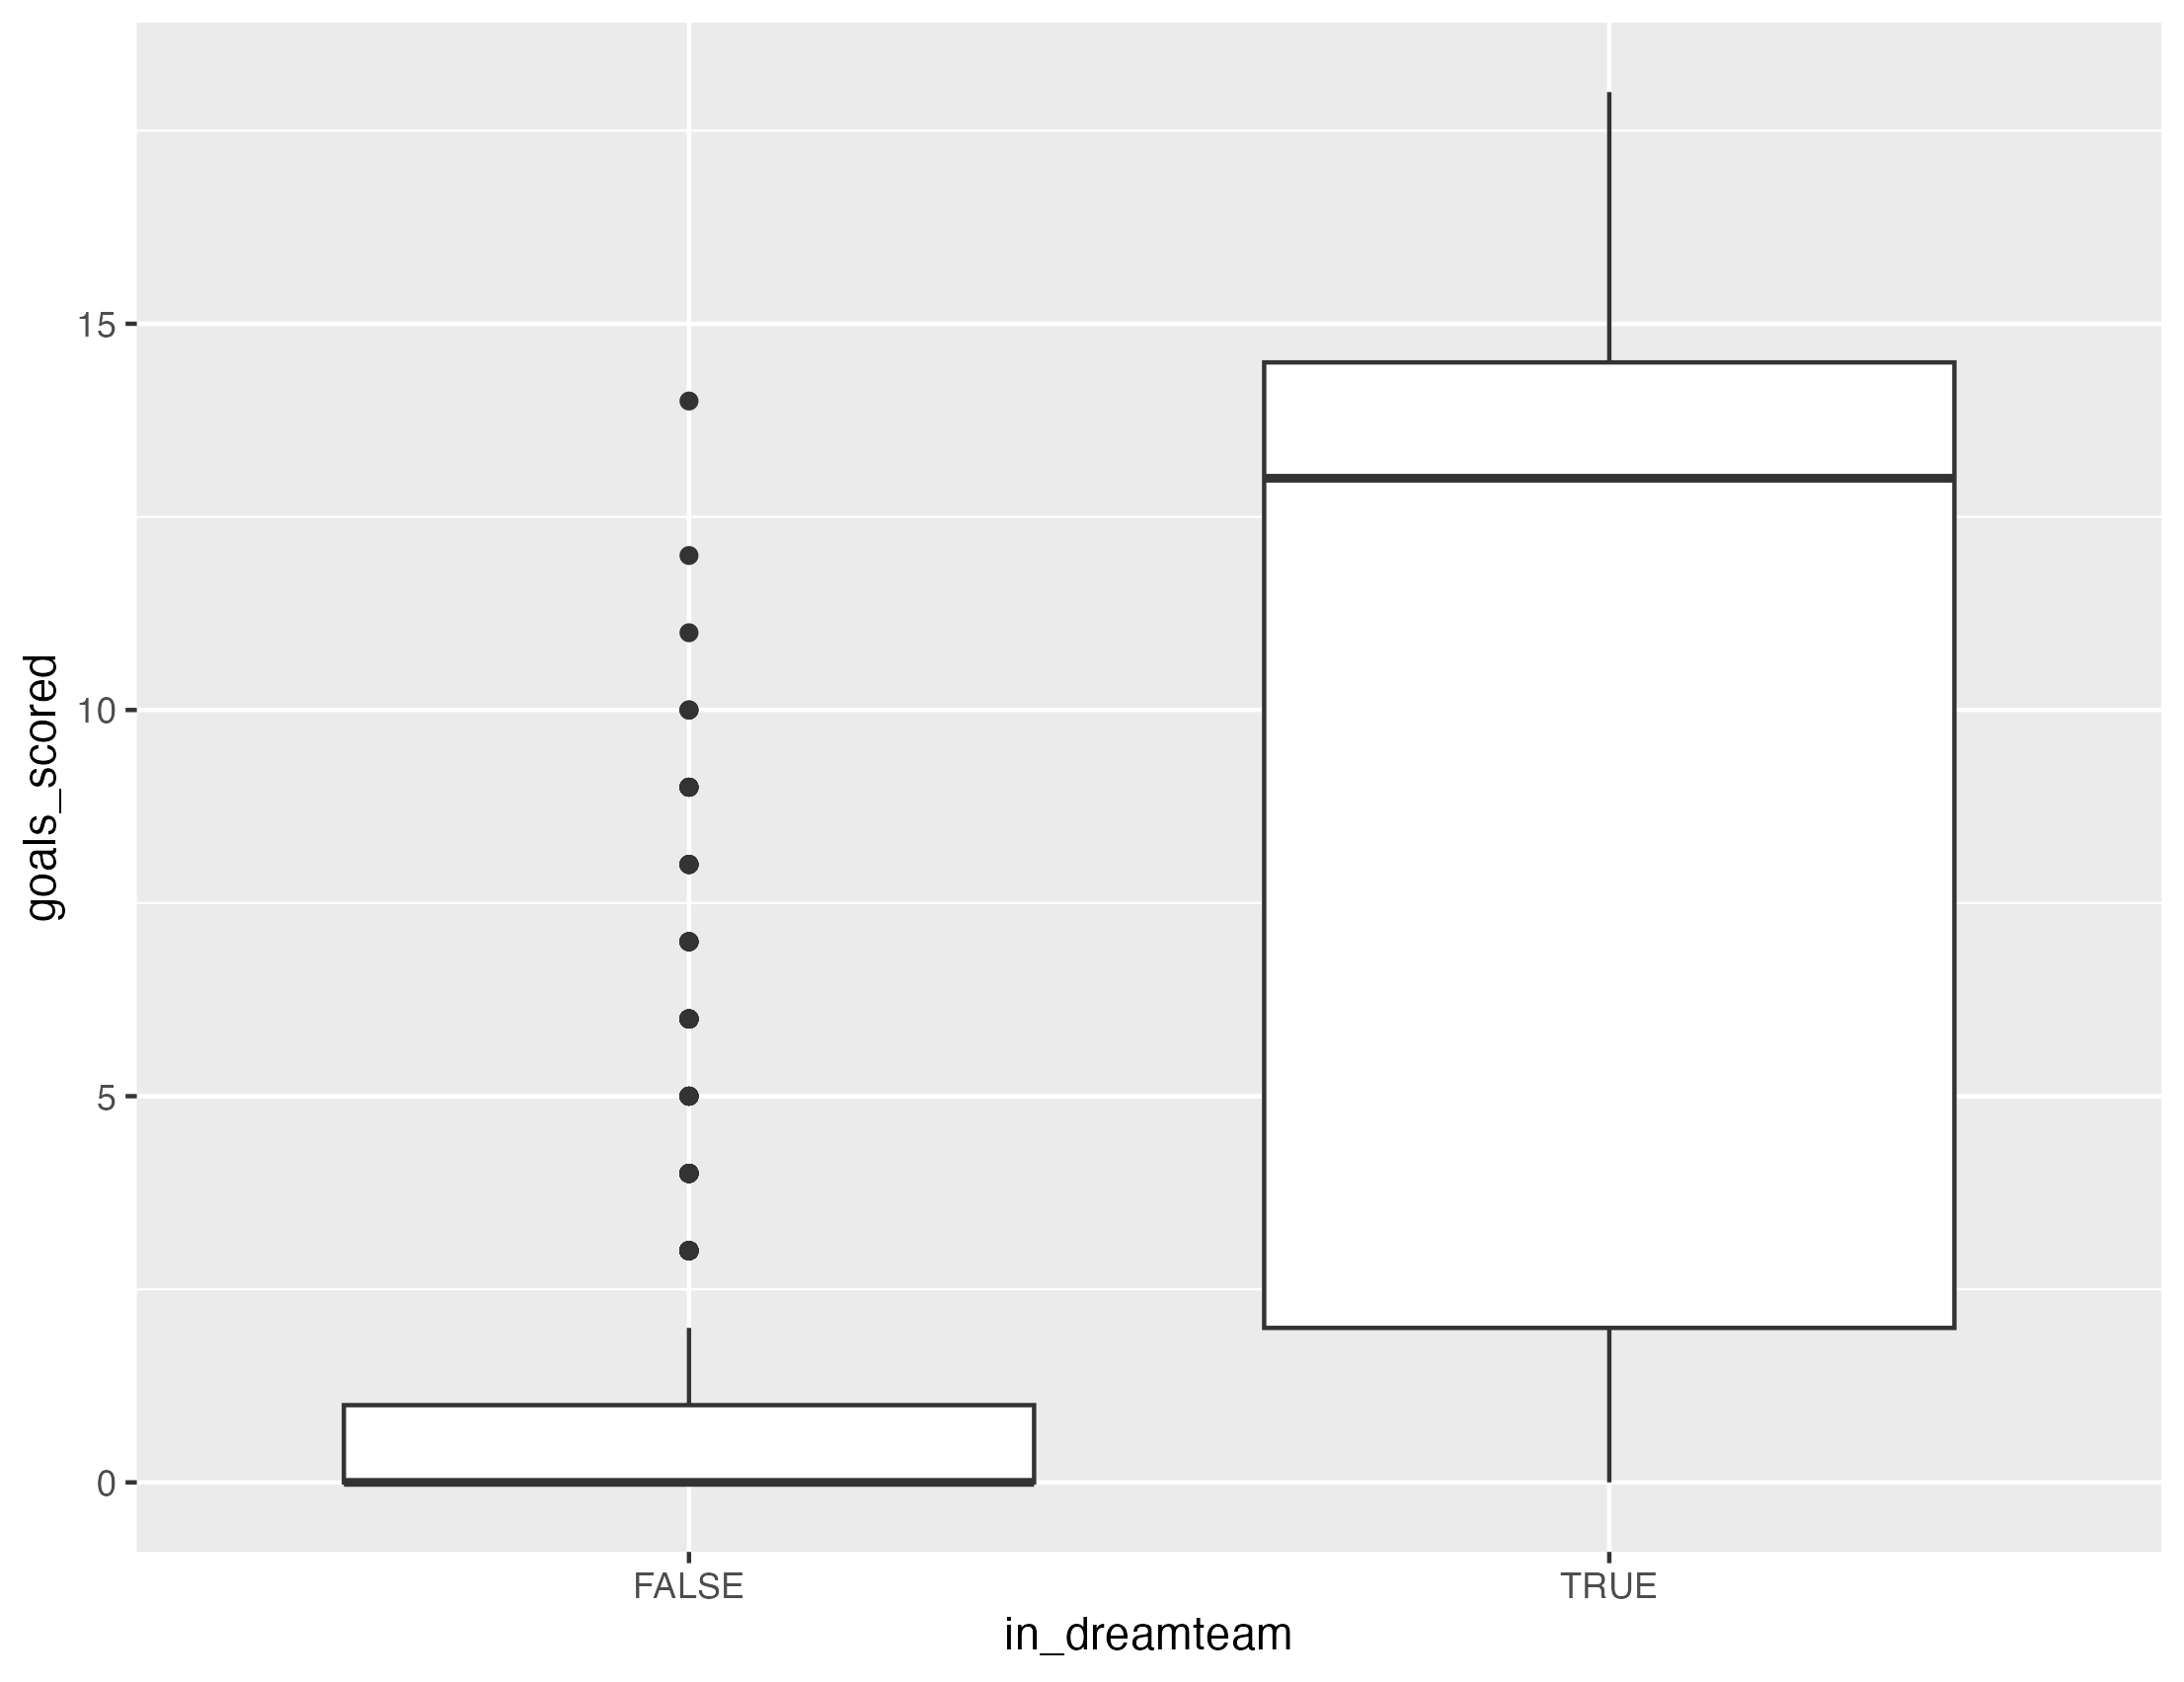
\includegraphics[width=0.75\linewidth]{PS6a_Akotenou.png}
\caption{\label{fig:frog}Goals scored per season given player's dream team.}
\end{figure}



\section{English Premiere League top 10 players} 
'Figure 2 shows the ten top EPL players based on their current market value. \textcolor{blue}{Haaland} is the most valuable player in the English Premier League, followed by \textcolor{blue}{Salah} and \textcolor{blue}{Kane}. Each of them costs more than £125 million sterling. \textcolor{blue}{De Bruyne} is the only player earning between £100 and £120 million sterling. \textcolor{blue}{Rashford, Odegaard}, and \textcolor{blue}{Alexander-Arnold} are those earning less than £25 million sterling in this category of players.'

\begin{figure}[H]
\centering
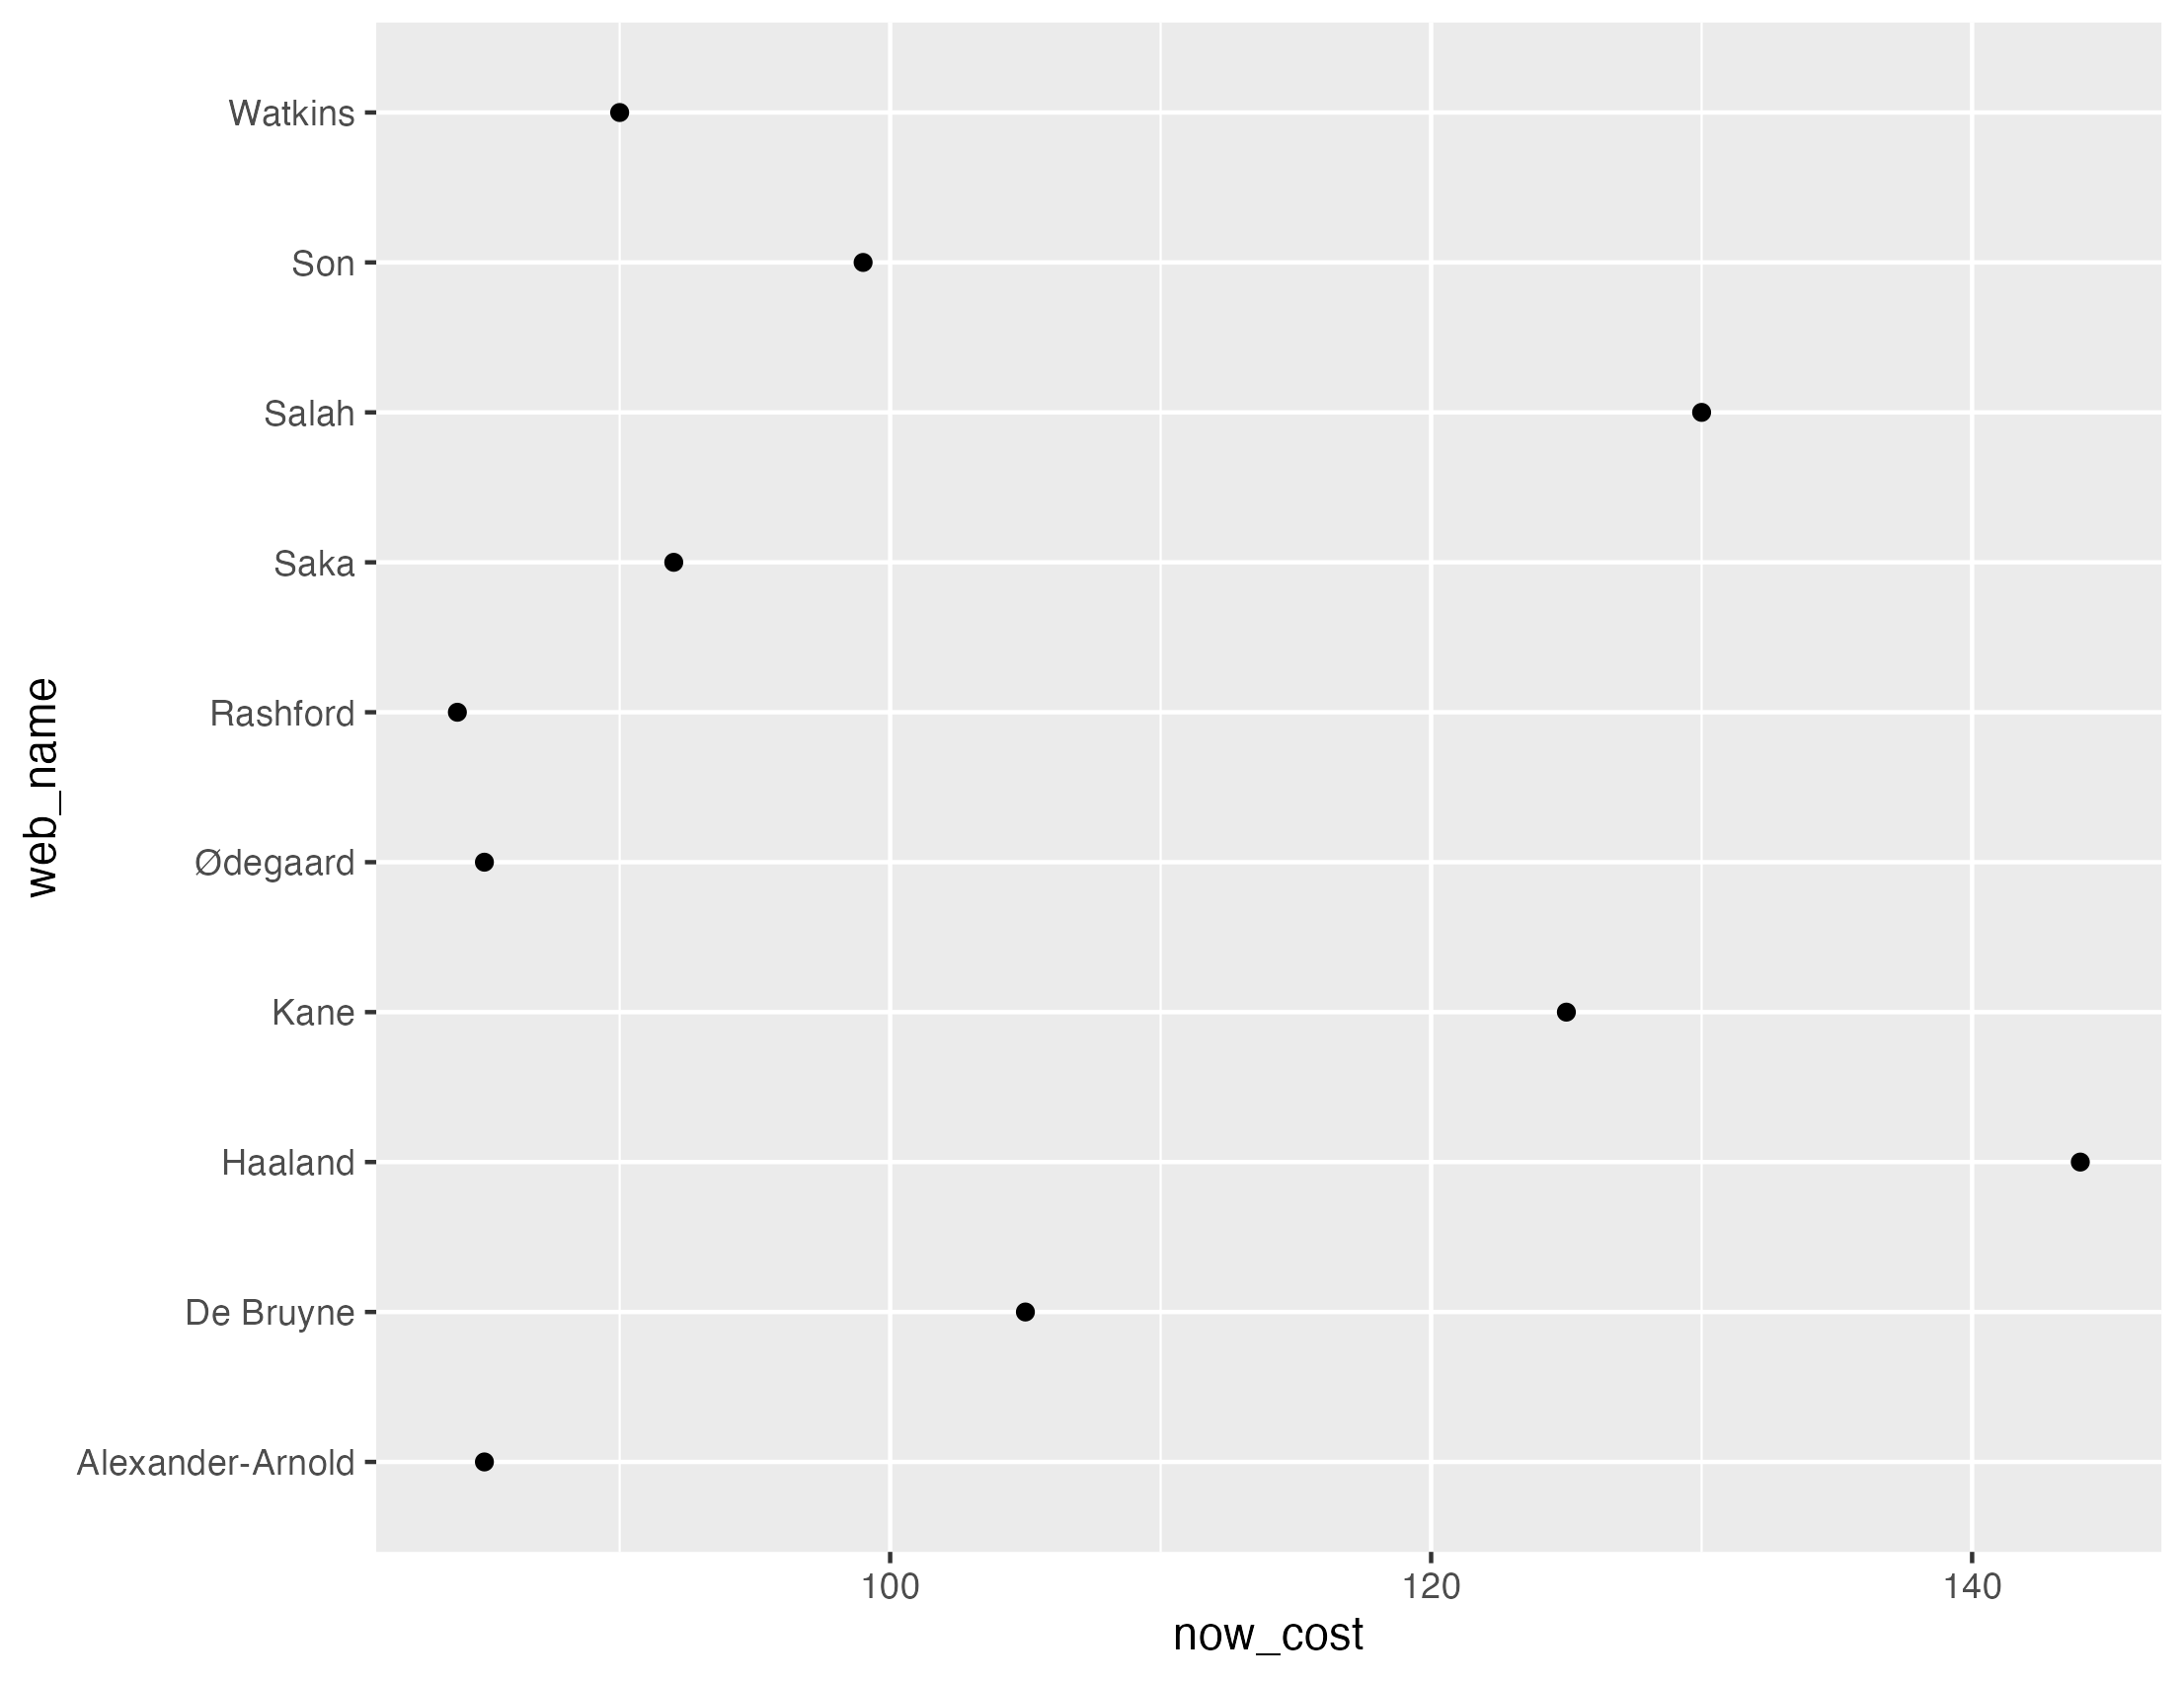
\includegraphics[width=0.75\linewidth]{PS6b_Akotenou.png}
\caption{\label{fig:frog}English Premiere League top 10 players.}
\end{figure}



\section{Relationship between performance and minutes playing on the field} 
In Figure 3, the number of goals scored is positively related to the number of minutes spent playing. Intuitively, this makes sense, as playing for more time increases the player's probability of scoring a goal.
\begin{figure}[H]
\centering
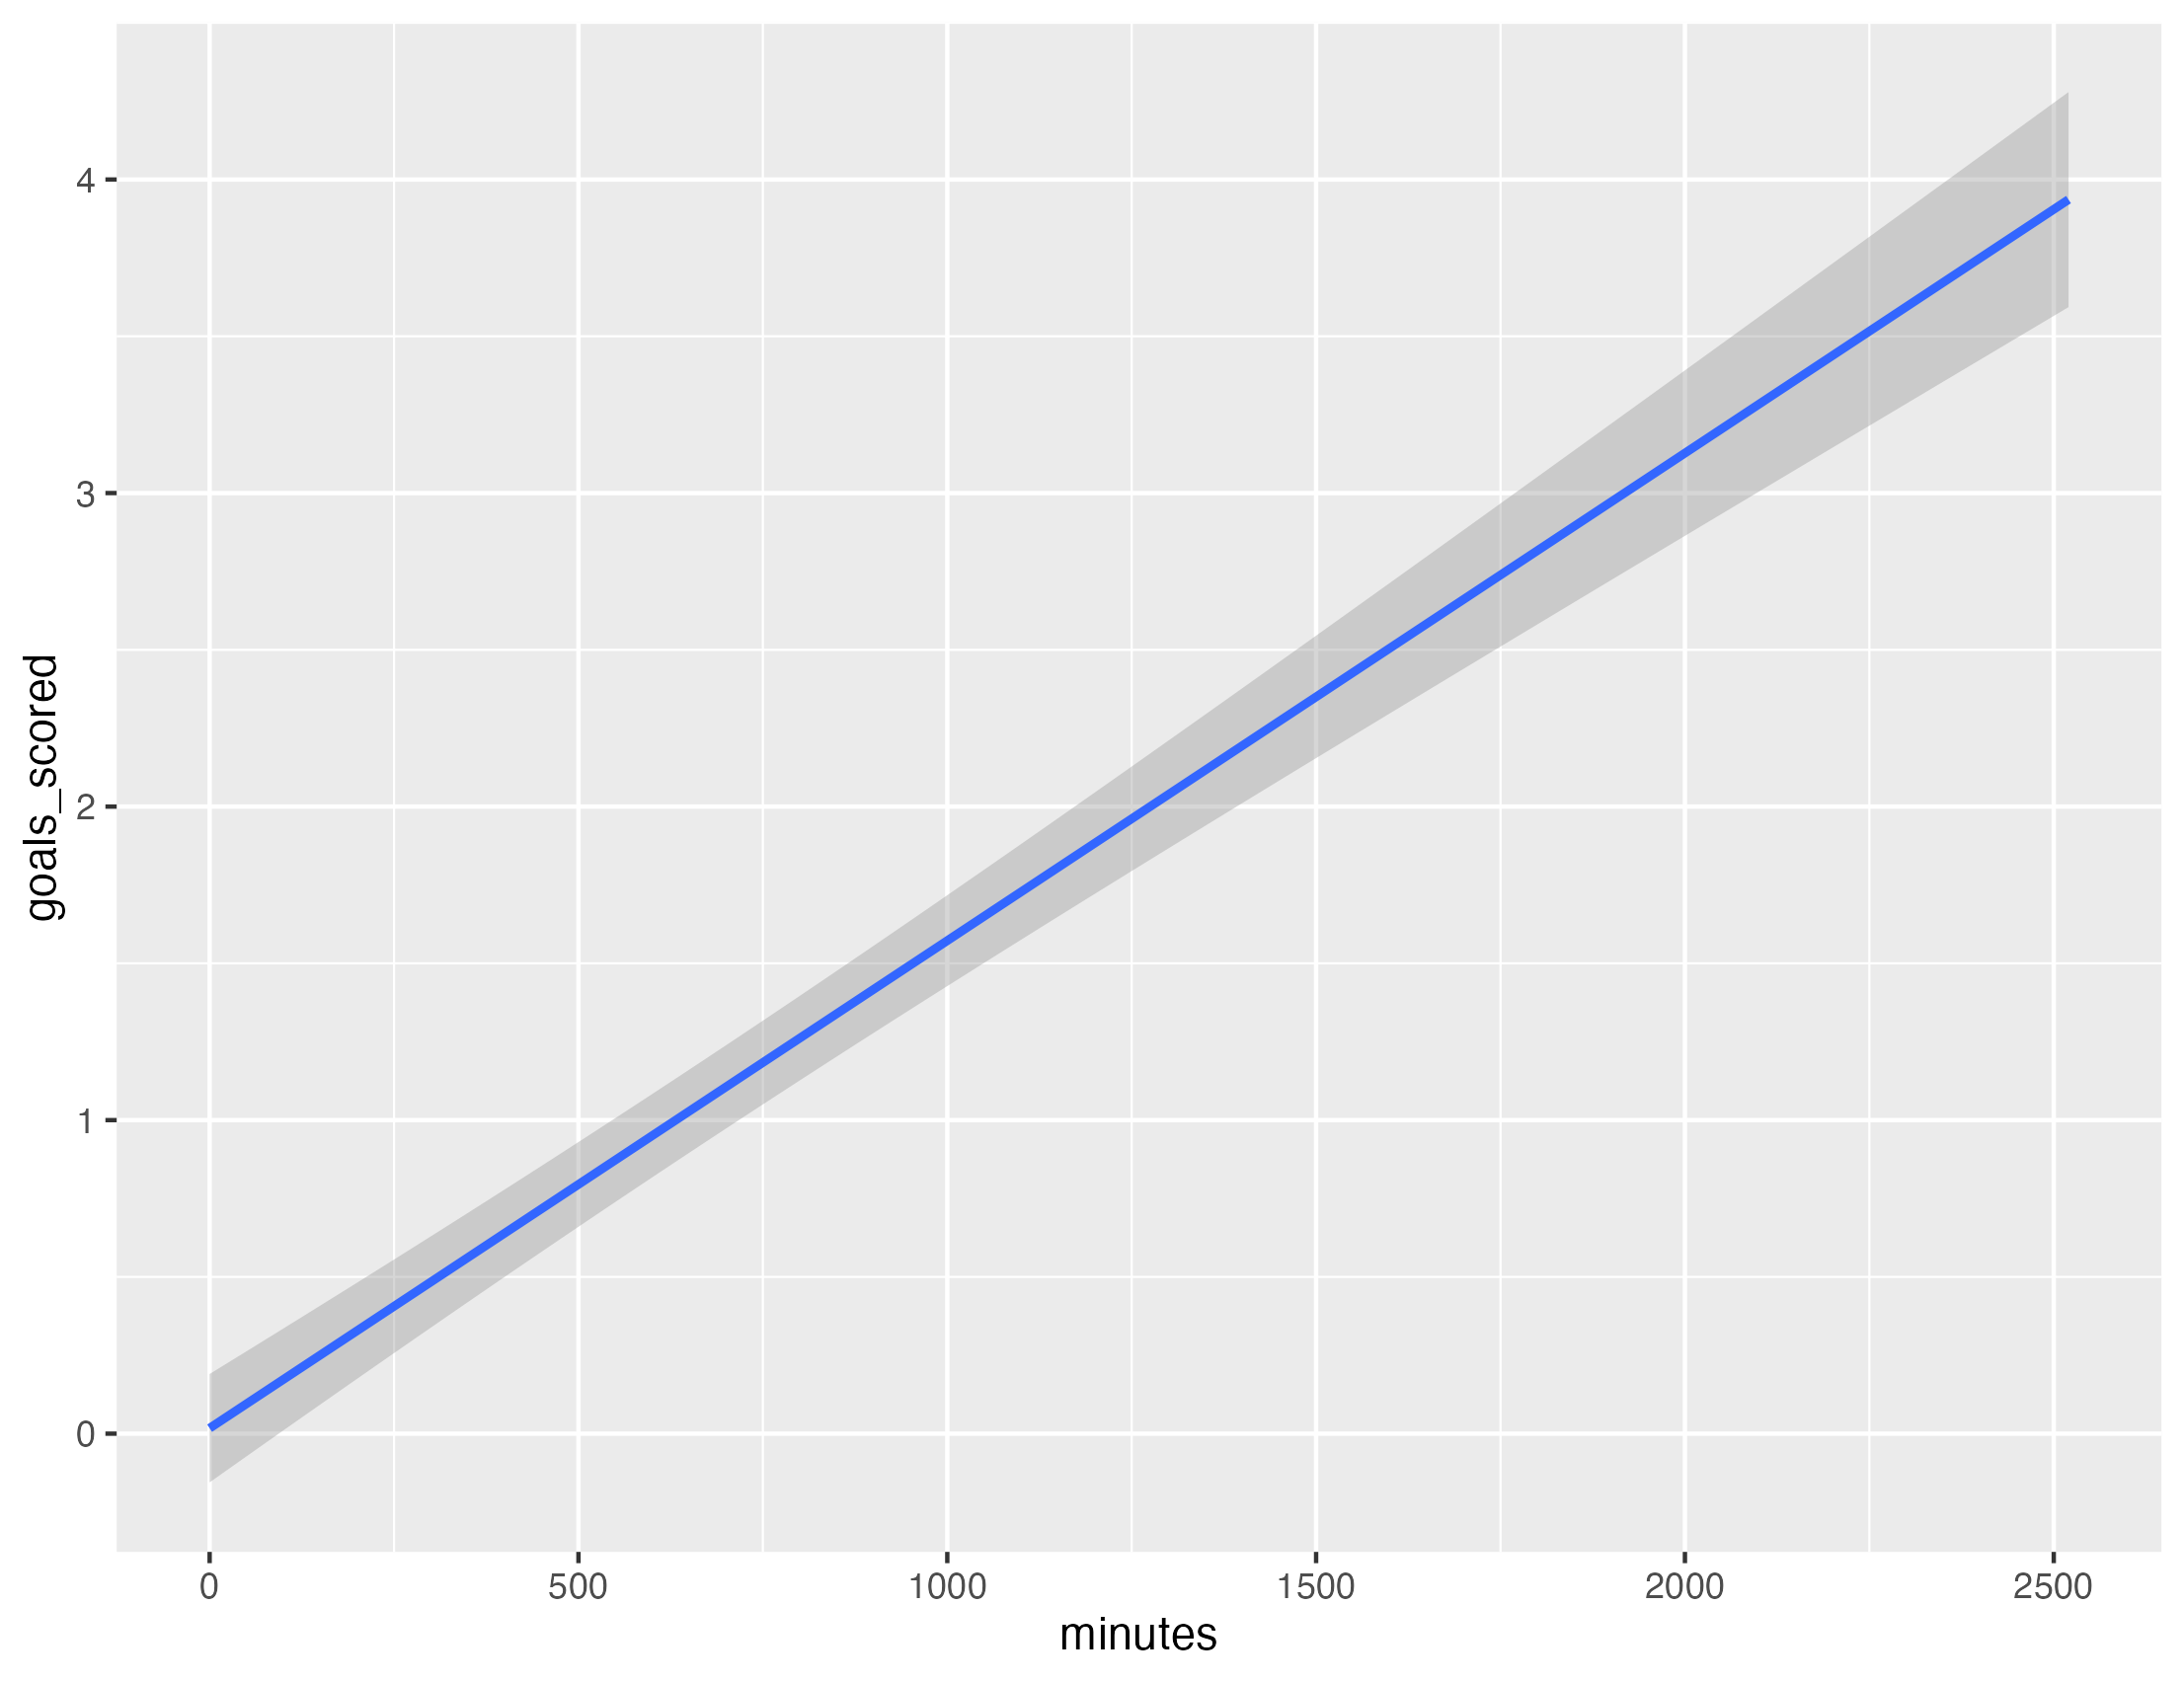
\includegraphics[width=0.75\linewidth]{PS6c_Akotenou.png}
\caption{\label{fig:frog}This frog was uploaded via the file-tree menu.}
\end{figure}





\end{document}